\documentclass[12pt, a4paper]{extarticle}
\usepackage[a4paper, margin=1.3cm]{geometry}
\usepackage[T1]{fontenc} % For polish characters in author name
\usepackage[utf8]{inputenc} % For global UTF-8 encoding
\usepackage{booktabs} % For "\specialrule" command
\usepackage{graphicx} % For graphics
\graphicspath{ {./images/} }
\usepackage{subfig} % For subfigures (images side by side)
\usepackage{amsmath} % For math
\usepackage{icomma} % For "intelligent" comma
\usepackage{multirow} % For generated table
\usepackage{float} % For table positioning
\usepackage{gensymb} % For degree symbol
%\usepackage{hyperref} % For hypertext links
\usepackage[bottom]{footmisc} % For footnotes on bottom of page
\usepackage[table,xcdraw]{xcolor} % For colored tables
\usepackage{multicol} % For multicolum lists
\usepackage[pdfusetitle]{hyperref} % For automatic PDF metadata
\usepackage[makeroom]{cancel} % For rossing out / canceling in math
\usepackage{pdflscape} % For landscape PDF
\usepackage{listings} % For source code listings (snippets)
\usepackage{svg} % For SVG graphics
\usepackage[super]{nth} % for "1st", "2nd" and "i-th" numbering: \nth{2}


%\usepackage[pdftex,
%pdfauthor={Kacper Jastrzębski, 260607@student.pwr.edu.pl},
%pdftitle={The Title},
%pdfsubject={The Subject},
%pdfkeywords={Some Keywords},
%pdfproducer={Latex with hyperref, or other system},
%pdfcreator={pdflatex, or other tool}]{hyperref} % For manual PDF metadata

\usepackage{letltxmacro} % For new style roots with "closing"
\makeatletter
\let\oldr@@t\r@@t
\def\r@@t#1#2{%
	\setbox0=\hbox{$\oldr@@t#1{#2\,}$}\dimen0=\ht0
	\advance\dimen0-0.2\ht0
	\setbox2=\hbox{\vrule height\ht0 depth -\dimen0}%
	{\box0\lower0.4pt\box2}}
\LetLtxMacro{\oldsqrt}{\sqrt}
\renewcommand*{\sqrt}[2][\ ]{\oldsqrt[#1]{#2} }
\makeatother

\renewcommand{\baselinestretch}{1.0}
%\renewcommand{\familydefault}{\sfdefault}
%\setlength{\parindent}{4em}
\setlength{\parskip}{0em}

\setlength{\arrayrulewidth}{0.2mm}
\setlength{\tabcolsep}{12pt}
\renewcommand{\arraystretch}{1.2}

\newcommand{\experiment}{E105}

% setting the line height in gather env.
\setlength{\jot}{3mm}


\title{
	Introduction to Robotics \\
	\vspace{\baselineskip}
	\large
	\textbf{Lecture 2}
}
\author{
	Kacper Jastrzębski\\
	260607@student.pwr.edu.pl
}
\date{Date: Tuesday 11:15, 7.03.2023}



\begin{document}

	\maketitle
	\vspace{1.5cm}

	\tableofcontents

	\pagebreak

	\begin{equation}
		R \in SO(3)
	\end{equation}

	\section{Elementary rotational matrices}



	\begin{equation}
		rot(z, \gamma) =
		\begin{bmatrix}
			\cos{\gamma} & -\sin{\gamma} & 0\\
			\sin{\gamma} & \cos{\gamma} & 0 \\
			0 & 0 & 1
		\end{bmatrix}
	\end{equation}

	\begin{equation}
		rot(y, \beta) =
		\begin{bmatrix}
			\cos{\beta} & 0 & \sin{\beta} \\
			0 & 1 & 0 \\
			-\sin{\beta} & 0 & \cos{\beta}
		\end{bmatrix}
	\end{equation}

	\begin{equation}
		rot(x, \alpha) =
		\begin{bmatrix}
			1 & 0 & 0\\
			0 & \cos{\alpha} & -\sin{\alpha} \\
			0 & \sin{\alpha} & \cos{\alpha}
		\end{bmatrix}
	\end{equation}

	\section{Representation of $R \in SO(3)$}

	\textbf{Roll-pitch-yaw} angles:
	\begin{equation}
		RPY(\alpha, \beta, \gamma) = rot(z, \alpha) \cdot rot(y, \beta)  \cdot rot(x, \gamma)
	\end{equation}
	\textbf{Euler} angles:
	\begin{equation}
		Euler(\alpha, \beta, \gamma) = rot(z, \alpha) \cdot rot(y, \beta)  \cdot rot(z, \gamma)
	\end{equation}

	\section{Operations on rotational matrices}

	\begin{equation}
		rot(x, \alpha) \cdot rot(z, \beta) \stackrel{?}{=} rot(z, \beta) \cdot rot(x, \alpha)
	\end{equation}

	Those two operations are \textbf{not} interchangeable, because matrix multiplication is not commutative.

	\begin{equation}
		R^n_0 = R^1_0 \cdot R^2_1 \cdots R^{n-1}_{n-2} \cdot R^n_{n-1}
	\end{equation}

	$p_n$ - position in n-th frame

	\begin{gather*}
		p_0 = R^1_0 \cdot p_n \\
		p_n = R^0_n \cdot p_0  \\
		p_0 = R^0_1 \cdot p_0 \\
		R^0_1 = (R^1_0)^{-1}=(R^1_0)^T
	\end{gather*}

	\begin{figure}[H]
		\centering
		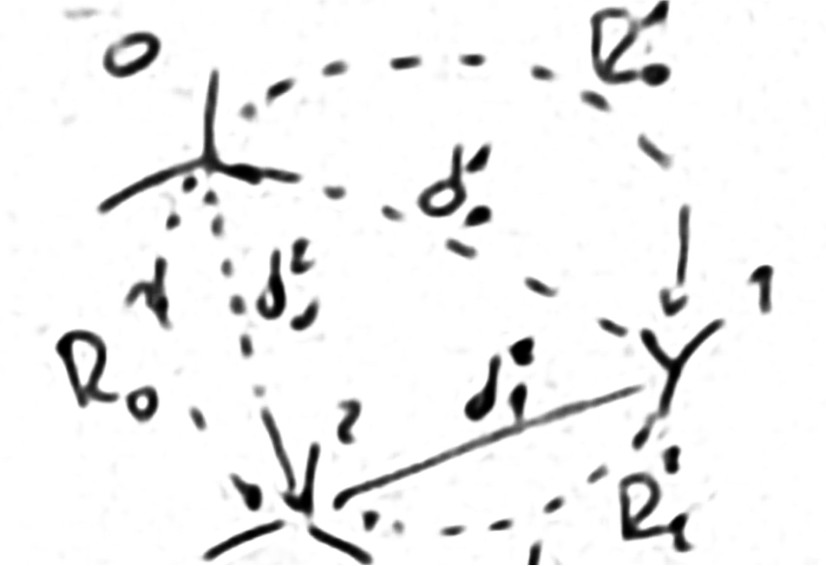
\includegraphics[width=10cm,trim={0 0 0 0},clip]{lecture-2-photo-1.jpg}
		\label{photo:1}%
	\end{figure}

	\begin{gather*}
		p_0 = p_1 + d^1_0  \text{(pure translation)} \\
		p_0 = R^1_0 \cdot p_1  \text{(pure rotation)} \\
		p_0 = R^1_0 p_1 + d^1_0 \\
		p_0 = R^2_0 p_2 + d^2_0 \\
		p_1 = R^2_1 p_2 + d^2_1
	\end{gather*}

	wh-1

\end{document}
